\chapter{Internet of Threads}                %crea il capitolo
%%%%%%%%%%%%%%%%%%%%%%%%%%%%%%%%%%%%%%%%%imposta l'intestazione di pagina
\lhead[\fancyplain{}{\bfseries\thepage}]{\fancyplain{}{\bfseries\rightmark}}
\pagenumbering{arabic}                  %mette i numeri arabi
\section{Paradigma}                 %crea la sezione
IoT (Internet of Things), ovvero l'internet delle cose.\\
Questo concetto vuole rapprensentare la diffusione dei sistemi embedded come veri e propri nodi di rete, possiamo definirlo il precursore del sistema che stiamo per descrivere ed \`e il sistema che ad oggi ha permesso di incontrare il nostro condizionatore o la nostra caldaia, ma addirittura il nostro tostapane, in rete.\\
Ad un certo punto si \`e sentita l'esigenza di elevare questa astrazione, nasce il concetto di IoTh.\\
L'idea diventa quella di avere processi come nodi di rete e non oggetti fisici, l'analogia \`e molto simile alla differenza tra telefoni fissi e telefoni cellulari, ovvero in passata era necessario pensare al luogo in cui una persona potesse trovarsi,, mentre attraverso l'assegnamento di un numero personale oggi possiamo comunicare direttamente con la persona desiderata\cite{K1,K2}.\\
In termini di internet questo si traduce nella possibilit\`a di migrare servizi da un capo all'altro del mondo con la semplicit\`a di un kill and start.\\
Come possiamo notare infatti, con questa tecnologia lo stack \`è direttamente integrato nel programma.
\begin{figure}[h]
\centering
\begin{minipage}{.5\textwidth}
\centering
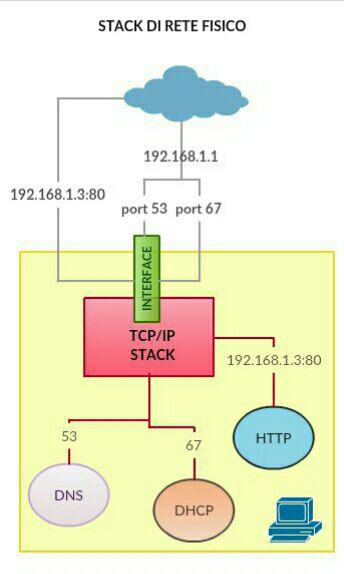
\includegraphics[width=7cm]{old_stack}
\caption[physical interface stack]{stack associato\\ all'interfaccia fisica}\label{fig:fisical}
\end{minipage}%
\begin{minipage}{.5\textwidth}
\centering
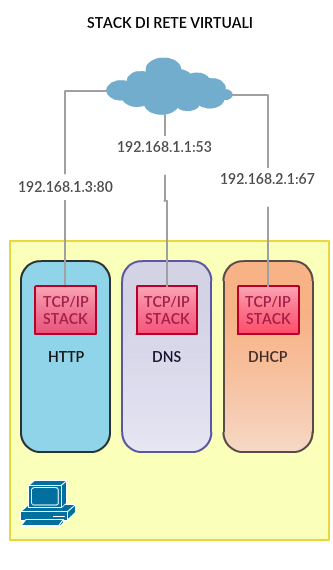
\includegraphics[width=7cm]{new_stack}
\caption[virtual stack]{stack associato\\ ai processi}\label{fig:virtual}
\end{minipage}
\end{figure}\\
Una nota va anche fatta in termini di sicurezza, ogni servizio pu\`o essere eseguito con il proprio stack di rete e questo impedirebbe a software di port mapping di carpire informazioni sulla macchina che ospita detto servizio. Inoltre possedendo il proprio stack di rete possiamo eseguire i processi con un utente non privilegiato e pertanto anche un bug del demone non comprometterebbe l'intero sistema.

\section{Stack Implementati}
Diversi sono i progetti che si occupano di offrire ai processi il proprio stack di rete; tra questi ne verranno presi in esame tre, considerati pi\`u indicati per uno studio in quanto open source, Ognuno di essi offre la propria implementazione di stack di rete.\\
Uno stack di rete legato al processo permette di connettere lo stesso ad una rete reale, tramite le interfacce fornite dal sistema, o virtuale (ad esempio VDE) come se fosse una macchina fisica a se stante, a questo punto ogni processo pu\`o staccarsi dal modo in cui la macchina che lo ospita gestisce la rete ed avere le proprie regole.\\

\subsection{PicoTCP}
Supportato da Tass Belgium (Altran); \`e lo stack pi\`u conosciuto e diffuso per sistemi embedded ed esistono anche dei progetti basati su IP di reti mesh realizzati con picoTCP\footnote{http://www.picotcp.com/mesh-design-guide}.
\subsection{LWIP}
Nasce dal progetto di Adam Dunkels pensato per sistemi embedded ed inizialmente non forniva supporto ad IPv6.\\
Light-weight IP vanta un core molto piccolo e la possibilit\`a di eseguire anche senza sistema oprativo (single-threaded) e con il minor consumo di RAM possibile, inoltre \`e modulare ed offre la possibilit\`a di aggiungere protocolli come DHCP e DNS solo in caso di necessit\`a.\\
Supporta sia little che big endian e gira su processori a 8 e 32 bit, quindi funziona anche su un semplice ATMEGA.\\
Unica pecca \`e il protoccolo IPv6 che \`e ancora in fase sperimentale, infatti il supporto IPv6 pu\`o essere aggiunto ed \`e scaricabile da git.
\subsection{LWIPv6}
Precedemente abbiamo fatto notare che LWIP non aveva supporto IPv6 e che tutt'ora \`e ancora in fase sperimentale, ed è questo uno dei motivi della nascita di LWIPv6.\\
Quando al team di virtual square \`e sopravvenuta la necessit\`a di avere uno stack per la rete vde non esisteva ancora nulla di maturo o comunque plug and play, da questa esigenza il team ha pensato di realizzare uno stack versatile in versione libreria tale per cui ogni processo potesse avere il proprio stack di rete.\\
Caratteristica principale di LWIPv6 \`e il suo motore ibrido che, di fatto funziona solo con IPv6 e mappa in questo protocollo le comunicazioni IPv4 utilizzando i primi 80 bit dell'indirizzo come flag di riconoscimento con tutti e 80 impostati a 1, ad esempio se volessimo rappresentare la maschera 255.255.255.0, che in esadecimale \`e equivalente a 0xffffff00 e la sua rappresentazione in IPv6 secondo LWIPv6 sar\`a la seguente 0xfffffff.ffffffff.ffffffff.ffffFFFF.ffffff00.
\section{Netlink}
Netlink \`e un sistema IPC (Inter Process Comunication) usato perch\`e in grado di mettere in comunicazione diversi task, solitamente serve per far comunicare task in user-space con task in kernel-space ma pu\`o far interagire anche processi entrambi in user-space.\\
Studiato per essere il successore di ioctl per le configurazioni ed il monitoraggio, si propone di essere pi\`u flessibile.
Ma come avviene esattamente la comunicazione attraverso netlink?\\
Netlink utilizza un sistema di socket indicizzato in base ai processi ogni processo pu\`o definire socket diversi di tipo netlink (AF\_NETLINK, NETLINK\_GENERIC, NETLINK\_XFRM) per inviare e ricevere messaggi con e da altri processi, implementa un sistema di porte basato sul process ID dei processi; ad esempio per la comunicazione con il kernel viene usata la porta 0.\\
L'immagine successiva rende perfettamente il concetto, ed \`e una rielaborazione (per puri motivi stilistici) dell'immagine della documtazione di libnl. (reperibile qui\footnote{https://www.infradead.org/~tgr/libnl/doc/images//addressing.png})
\begin{figure}[h]                       %crea l'ambiente figura; [h] sta
                                        %   per here, cio� la figura va qui
\begin{center}                          %centra nel mezzo della pagina
                                        %   la figura
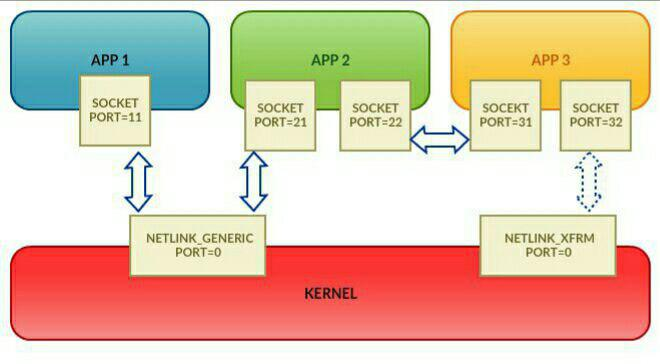
\includegraphics[width=15cm]{netlink_comunication}%inserisce una figura larga 5cm
                                        %se si vuole usare va scommentata
%
%%%%%%%%%%%%%%%%%%%%%%%%%%%%%%%%%%%%%%%%%inserisce la legenda ed etichetta
                                        %   la figura con \label{fig:prima}
\caption[scambio di messaggi attraverso socket netlink]{comunicazione netlink}
\end{center}
\end{figure}
L'interfaccia di comunicazione \`e abbastanza standardizzata ma personalizzabile a livello di payload, ognuno pu\`o definire una struttura personalizzata per poi usarla per comunicare attraverso i socket netlink con altri processi.
\subsection{Inter Process Comunication}
Molti processi necessitano di scambiare informazioni per i motivi pi\`u disparati, dalla comunicazion e di rete a quella interna ad una sola macchina.\\
Viene da se pensare che costruire programmi che non interagiscono con il mondo esterno o con altri programmi sarebbe una risorsa limitata.\\
Con IPC intendiamo quindi l'insieme delle tecnologie adottate per permettere ai processi di comunicare tra essi, che siano ospitati sulla stessa macchina o distribuiti sulla rete, tra queste tecnologie esiste appunto quella utilizzata all'interno della libreria oggetto di questo elaborato.
\subsection{Libnl}
Netlink Protocol Library Suite (libnl), \`e una raccolta di librerie ed utility che forniscono API di comunicazione netlink basate su quelle del kernel linux e comprende \cite{K10}:
\begin{description}                     %crea un elenco descrittivo
  \item[libnl] Core della libreria, offre uno strato di unificazione delle interfacce sulle quali poi si basano le altre librerie che pertanto di pendo da questa;
  \item[libnl-route] Questa libreria si occupa di fornire API per la configurazione degli elemnti della famiglia NETLINK\_ROUTE;
  \item[libnl-genl] genl significa generic netlink e questa libreria offre una versione estesa del protocollo netlink;
  \item[libnl-nf] API per configurazioni netlink basate su netfilter.

\end{description}
%%%%%%%%%%%%%%%%%%%%%%%%%%%%%%%%%%%%%%%%%non numera l'ultima pagina sinistra

\clearpage{\pagestyle{empty}\cleardoublepage} 
